\begin{frame}{Secret Sharing $L_\infty$ ball}
    \begin{itemize}
        \item For center $(x_1, \ldots, x_d)$, we want to secret share this huge $L_\infty$ ball:
        \begin{equation*}
            [x_1 - \delta, x_1 + \delta] \times [x_2 - \delta, x_2 + \delta] \times \ldots \times [x_n - \delta, x_n + \delta]
        \end{equation*}

        \visible<2>{
        \item We can secret share each dimension separately, then AND the results.
        \begin{equation*}
            x_1 + \delta \ge y_1 \ge x_1 - \delta \quad \wedge \quad \ldots \quad \wedge \quad x_d + \delta \ge y_d \ge x_d - \delta
        \end{equation*}
        }

    \end{itemize}

    \centering
    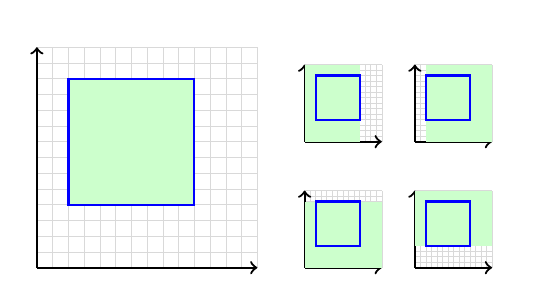
\begin{tikzpicture}[scale=0.4]
        % light grid
        \draw[step=0.5cm,gray!30,very thin] (0, 0) grid (7, 7);
    
        % axes
        \draw[->,thick] (0,0) -- (7,0) node[right] {};
        \draw[->,thick] (0,0) -- (0,7) node[above] {};
    
        % square with corners (1,2) and (5,6)
        \draw[thick,blue,fill=green!20] (1,2) rectangle (5,6);
    
        % optional: mark the corners
        % \filldraw[blue] (1,2) circle (2pt);
        % \filldraw[blue] (5,6) circle (2pt);
    
        % small planes on the right (2x2)
        \visible<2>{
        \begin{scope}[xshift=8.5cm,yshift=4cm,scale=0.35]
            \draw[step=0.5cm,gray!30,very thin] (0, 0) grid (7, 7);
            \draw[->,thick] (0,0) -- (7,0) node[right] {};
            \draw[->,thick] (0,0) -- (0,7) node[above] {};
            \fill[green!20] (0,0) rectangle (5,7);
            \draw[thick,blue] (1,2) rectangle (5,6);
        \end{scope}
        \begin{scope}[xshift=12cm,yshift=4cm,scale=0.35]
            \draw[step=0.5cm,gray!30,very thin] (0, 0) grid (7, 7);
            \draw[->,thick] (0,0) -- (7,0) node[right] {};
            \draw[->,thick] (0,0) -- (0,7) node[above] {};
            \fill[green!20] (1,0) rectangle (7,7);
            \draw[thick,blue] (1,2) rectangle (5,6);
        \end{scope}
        \begin{scope}[xshift=8.5cm,yshift=0cm,scale=0.35]
            \draw[step=0.5cm,gray!30,very thin] (0, 0) grid (7, 7);
            \draw[->,thick] (0,0) -- (7,0) node[right] {};
            \draw[->,thick] (0,0) -- (0,7) node[above] {};
            \fill[green!20] (0,0) rectangle (7,6);
            \draw[thick,blue] (1,2) rectangle (5,6);
        \end{scope}
        \begin{scope}[xshift=12cm,yshift=0cm,scale=0.35]
            \draw[step=0.5cm,gray!30,very thin] (0, 0) grid (7, 7);
            \draw[->,thick] (0,0) -- (7,0) node[right] {};
            \draw[->,thick] (0,0) -- (0,7) node[above] {};
            \fill[green!20] (0,2) rectangle (7,7);
            \draw[thick,blue] (1,2) rectangle (5,6);
        \end{scope}
        }
    \end{tikzpicture}

\end{frame}
% Note: In the script, state clearly that in this talk to keep things simple, we do not talk about overflow

\begin{frame}
    \frametitle{Primitive: Function Secret Sharing (FSS)}
    \begin{itemize}
        \item FSS was introduced in \cite{boyle2015function}, allowing to secret share a function $f$ between multiple parties.
        \item For domain bit length $u$, security parameter $\kappa$, payload bit length $v$, the key size is $O(u \cdot (\kappa + v))$ bits.
    \end{itemize}
    \begin{center}
    \vspace{-1cm}
    \begin{tikzpicture}[>=stealth,thick,scale=0.9]
        \node[minimum width=1.5cm,minimum height=1.2cm,align=center] (interval) at (-0.3,0) {$x_1 + \delta \ge y_1 \ge x_1 - \delta?$\footnote{We actually need to concatenate two FSSs. More details are found in the paper.}};
        \node (oracle) at (3,0) {\includegraphics[width=2cm]{images/crystal_ball_transparent.png}};
        \node (key1) at (6,1.4) {\includegraphics[width=1.8cm]{images/key_transparent.png}};
        \node (key0) at (6,-1.4) {\includegraphics[width=1.8cm]{images/key_transparent.png}};
        \node (mag1) at (8,1.4) {\includegraphics[width=1.2cm]{images/magnifier_transparent.png}};
        \node (mag0) at (8,-1.5) {\includegraphics[width=1.2cm]{images/magnifier_transparent.png}};
        \node at ([xshift=-0.1cm,yshift=0.1cm]mag1) {$y_1$};
        \node at ([xshift=-0.1cm,yshift=0.1cm]mag0) {$y_1$};

        \node[anchor=west] (b1) at (9,1.4) {$b_1$};
        \node[anchor=west] (b0) at (9,-1.4) {$b_0$};
        \node[anchor=west,align=left,text width=5cm] (cases) at (10,0) {$\begin{cases}
            b_0 = b_1 \text{ if } y_1 \le x_1 - \delta \\
            b_0 \neq b_1 \text{ if } y_1 > x_1 - \delta
        \end{cases}$};

        \draw[->] (interval.east) -- ([xshift=0.2cm]oracle.west);
        \draw[->] (oracle.east) -- (key1.west);
        \draw[->] (oracle.east) -- (key0.west);
        \draw[->] (key1.east) -- (mag1.west);
        \draw[->] (key0.east) -- ([yshift=0.1cm]mag0.west);
        \draw[->] (mag1.east) -- (b1.west);
        \draw[->] ([yshift=0.1cm]mag0.east) -- (b0.west);
        \draw[->] (b1.east) -- (cases.west);
        \draw[->] (b0.east) -- (cases.west);

        \node at ([yshift=-8pt]key1.north) {$k_1$};
        \node at ([yshift=8pt]key0.south) {$k_0$};
        \node at (mag1.north) {$k_1.\mathrm{Eval}(y_1)$};
        \node at ([yshift=0.05cm]mag0.south) {$k_0.\mathrm{Eval}(y_1)$};
    \end{tikzpicture}
    \end{center}
\end{frame}

\begin{frame}
    \frametitle{Function Secret Sharing in \cite{garimella2024computation}}
    \begin{itemize}
        \item Alice prepares $O(\kappa)$ FSS keys pairs with \textit{binary output} (\textit{in} / \textit{out}?) for each inequality check.
        \visible<2>{
        \item Alice and Bob runs 1-out-of-2 OTs, for Bob to learn either $k_0^i$ or $k_1^i$.
        \item If the inequality check succeeds, for any of $\kappa$ key pairs, the evaluations would be equal.
        }
    \end{itemize}
    \begin{center}
    \begin{tikzpicture}[>=stealth,thick,node distance=0.9cm and 1.4cm,xscale=0.95]
        \node[anchor=west] (alice) at (-1.2,2) {\includegraphics[height=1.6cm]{images/Alice_transparent.png}};
        \node (ineq) at (0,0) {$y_1 \ge x_1 - \delta\ ?$};

        % hardcoded key pairs instead of loop
        % columns for keys are closer together; OT sits to the right with arrow from midpoint
        \node (k01) at (3.2,2.4) {$k_0^{1,1}$};
        \node (k11) at (3.2,1.8) {$k_1^{1,1}$};

        \node (k02) at (3.2,0.9) {$k_0^{1,2}$};
        \node (k12) at (3.2,0.3) {$k_1^{1,2}$};

        \node (k0dots) at (3.2,-0.5) {$\vdots$};

        \node (k0k) at (3.2,-1.6) {$k_0^{1,\kappa}$};
        \node (k1k) at (3.2,-2.2) {$k_1^{1,\kappa}$};

        % wiring from inequality to keys (always visible)
        \foreach \n in {k01,k11,k02,k12,k0k,k1k}{
            \draw[->] (ineq.east) -- (\n.west);
        }

        \coordinate (mid1) at (3.6,2.1);
        \coordinate (mid2) at (3.6,0.6);
        \coordinate (midk) at (3.6,-1.9);

        % OT boxes and arrows appear only on the second overlay
        \visible<2>{
            \node[draw,rounded corners,fill=gray!15,inner sep=4pt] (ot1) at (5.6,2.1) {OT};
            \node[draw,rounded corners,fill=gray!15,inner sep=4pt] (ot2) at (5.6,0.6) {OT};
            \node[draw,rounded corners,fill=gray!15,inner sep=4pt] (otk) at (5.6,-1.9) {OT};

            \draw[->] (mid1) -- (ot1.west);
            \draw[->] (mid2) -- (ot2.west);
            \draw[->] (midk) -- (otk.west);
        }

        \node[anchor=west] (bob) at (9.2,2) {\includegraphics[height=1.4cm]{images/Bob transparent.png}};
        \visible<2>{
            \draw[->] (ot1.east) -- (bob.west);
            \draw[->] (ot2.east) -- (bob.west);
            \draw[->] (otk.east) -- (bob.west);
        }
    \end{tikzpicture}
    \end{center}
\end{frame}

\begin{frame}
    \frametitle{Sneak peak: How to find intersection?}
    \begin{itemize}
        \item Setup: In the $j^{\mathrm{th}}$-th OT of the $i^{\mathrm{th}}$ dimension, Bob receives $k_{c_{i,j}}^{i,j}$, where $c_{i,j}$ is the OT choice.
        \item For each Bob's element $y$, with dimensions $1, 2, \ldots, d$, Bob can compute:
        \begin{equation*}
        \begin{aligned}
            \mathsf{H} (& k_{c_{1,1}}^{1,1}.\mathrm{Eval}(y_1) \| k_{c_{1,2}}^{1,2}.\mathrm{Eval}(y_1) \| \ldots \| k_{c_{1,\kappa}}^{1,\kappa}.\mathrm{Eval}(y_1) \\
            &\| k_{c_{2,1}}^{2,1}.\mathrm{Eval}(y_2) \| k_{c_{2,2}}^{2,2}.\mathrm{Eval}(y_2) \| \ldots \| k_{c_{2,\kappa}}^{2,\kappa}.\mathrm{Eval}(y_2) \\
            &\| \vdots \\
            &\| k_{c_{d,1}}^{d,1}.\mathrm{Eval}(y_d) \| k_{c_{d,2}}^{d,2}.\mathrm{Eval}(y_d) \| \ldots \| k_{c_{d,\kappa}}^{d,\kappa}.\mathrm{Eval}(y_d) )
        \end{aligned}
        \end{equation*}
        \item For each Alice's element, simply evaluate with the first key:
        \begin{equation*}
        \begin{aligned}
            \mathsf{H} (& k_{0}^{1,1}.\mathrm{Eval}(y_1) \| k_{0}^{1,2}.\mathrm{Eval}(y_1) \| \ldots \| k_{0}^{1,\kappa}.\mathrm{Eval}(y_1) \\
            &\| k_{0}^{2,1}.\mathrm{Eval}(y_2) \| k_{0}^{2,2}.\mathrm{Eval}(y_2) \| \ldots \| k_{0}^{2,\kappa}.\mathrm{Eval}(y_2) \\
            &\| \vdots \\
            &\| k_{0}^{d,1}.\mathrm{Eval}(y_d) \| k_{0}^{d,2}.\mathrm{Eval}(y_d) \| \ldots \| k_{0}^{d,\kappa}.\mathrm{Eval}(y_d) )
        \end{aligned}
        \end{equation*}
        \item If $y$ is inside the $L_\infty$ ball, all evaluations would be equal.
    \end{itemize}
\end{frame}

\begin{frame}
    \frametitle{Why do we need $\kappa$ key pairs?}
    \begin{itemize}
        \item If the hash input's entropy is low, Alice can do \textit{dictionary attack}.
        \visible<2,3>{
        \item Alice can prepare only one FSS key pair for each inequality check, with \textit{longer payload}.
        \item However, Alice knows the payload, which is undesirable.
        }
        \visible<3>{
        \item Nonetheless, the key size for one inequality check is improved:
        }
    \end{itemize}
    \visible<3>{
    \centering
    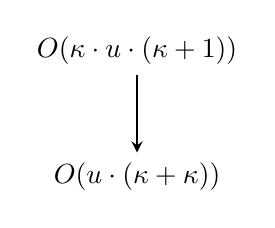
\begin{tikzpicture}[>=stealth,thick]
        \node (eqtop) at (0,0) {$O(\kappa \cdot u \cdot (\kappa + 1))$};
        \node (eqbottom) at (0,-1.6) {$O(u \cdot (\kappa + \kappa))$};
        \draw[->] (eqtop) -- (eqbottom);
    \end{tikzpicture}
    }
\end{frame}

\begin{frame}
    \frametitle{Distributed DCF}
    \begin{itemize}
        \item To hide the payload from Alice, we let Bob choose it!
    \end{itemize}
    \begin{center}
    \begin{tikzpicture}[>=stealth,thick]
        % parties
        \node[anchor=west] (alice) at (0,2.8) {\includegraphics[height=1.6cm]{images/Alice_transparent.png}};
        \node[anchor=west] (bob)   at (10,2.8) {\includegraphics[height=1.6cm]{images/Bob transparent.png}};

        % inputs
        \node[anchor=north,align=center] (ainterval) at ([yshift=-0.2cm]alice.south) {$[x_1-\delta,\,x_1+\delta]$};
        \node[anchor=north,align=center] (binput) at ([yshift=-0.2cm]bob.south) {$\beta$};

        % oracle
        \node (oracle) at (5.5,0.8) {\includegraphics[width=2.4cm]{images/crystal_ball_transparent.png}};

        % outputs
        \node[anchor=north] (k0) at ([yshift=-2cm]alice.south) {$k_0$};
        \node[anchor=north] (k1) at ([yshift=-2cm]bob.south) {$k_1$};

        % wiring
        \draw[->] (ainterval.south) -- ([xshift=-0.4cm]oracle.west);
        \draw[->] (binput.south) -- ([xshift=0.4cm]oracle.east);
        \draw[->] ([yshift=-0.6cm,xshift=-0.4cm]oracle.west) -- (k0.east);
        \draw[->] ([yshift=-0.6cm,xshift=0.4cm]oracle.east) -- (k1.west);
    \end{tikzpicture}
    \end{center}
    \begin{itemize}
        \item Alice and Bob are now ready for the searching phase!
    \end{itemize}
\end{frame}
